\section{一些真实的分布}

\subsection{几何}
\subsubsection{随机向量夹角的分布}
对于$\mathbb{R}^n$空间,(从均匀分布)随机取两个向量,则夹角的概率分布为
$$p(\theta)=\frac{\Gamma \left(\frac{n}{2}\right)}{\Gamma \left(\frac{n-1}{2}\right)}\frac{\sin^{n-2}(\theta)}{\sqrt{\pi}}$$

当$n=2$时,$p(\theta)=\frac{1}{\pi}$。

当$n=3$时,$p(\theta)=\frac{1}{2}\sin\theta$。

推导也比较容易,首先任意取一个向量,然后另一个向量与它形成夹角$\theta$,夹角增加$\dif\theta$在球面上切割出环状区域,面积$\Delta S$,这个区域的面积与整个球的表面积之和,即为概率密度,即
$$p(\theta)\dif\theta=\frac{\Delta S}{S_{n-1}}=\frac{S_{n-2}(R\sin\theta)R\dif\theta}{S_{n-1}(R)}$$
注意环的内圆就是$n-2$维球。$n$维球的表面积公式参见\ref{ndsphere}。在三维空间中比较直观:
\begin{center}
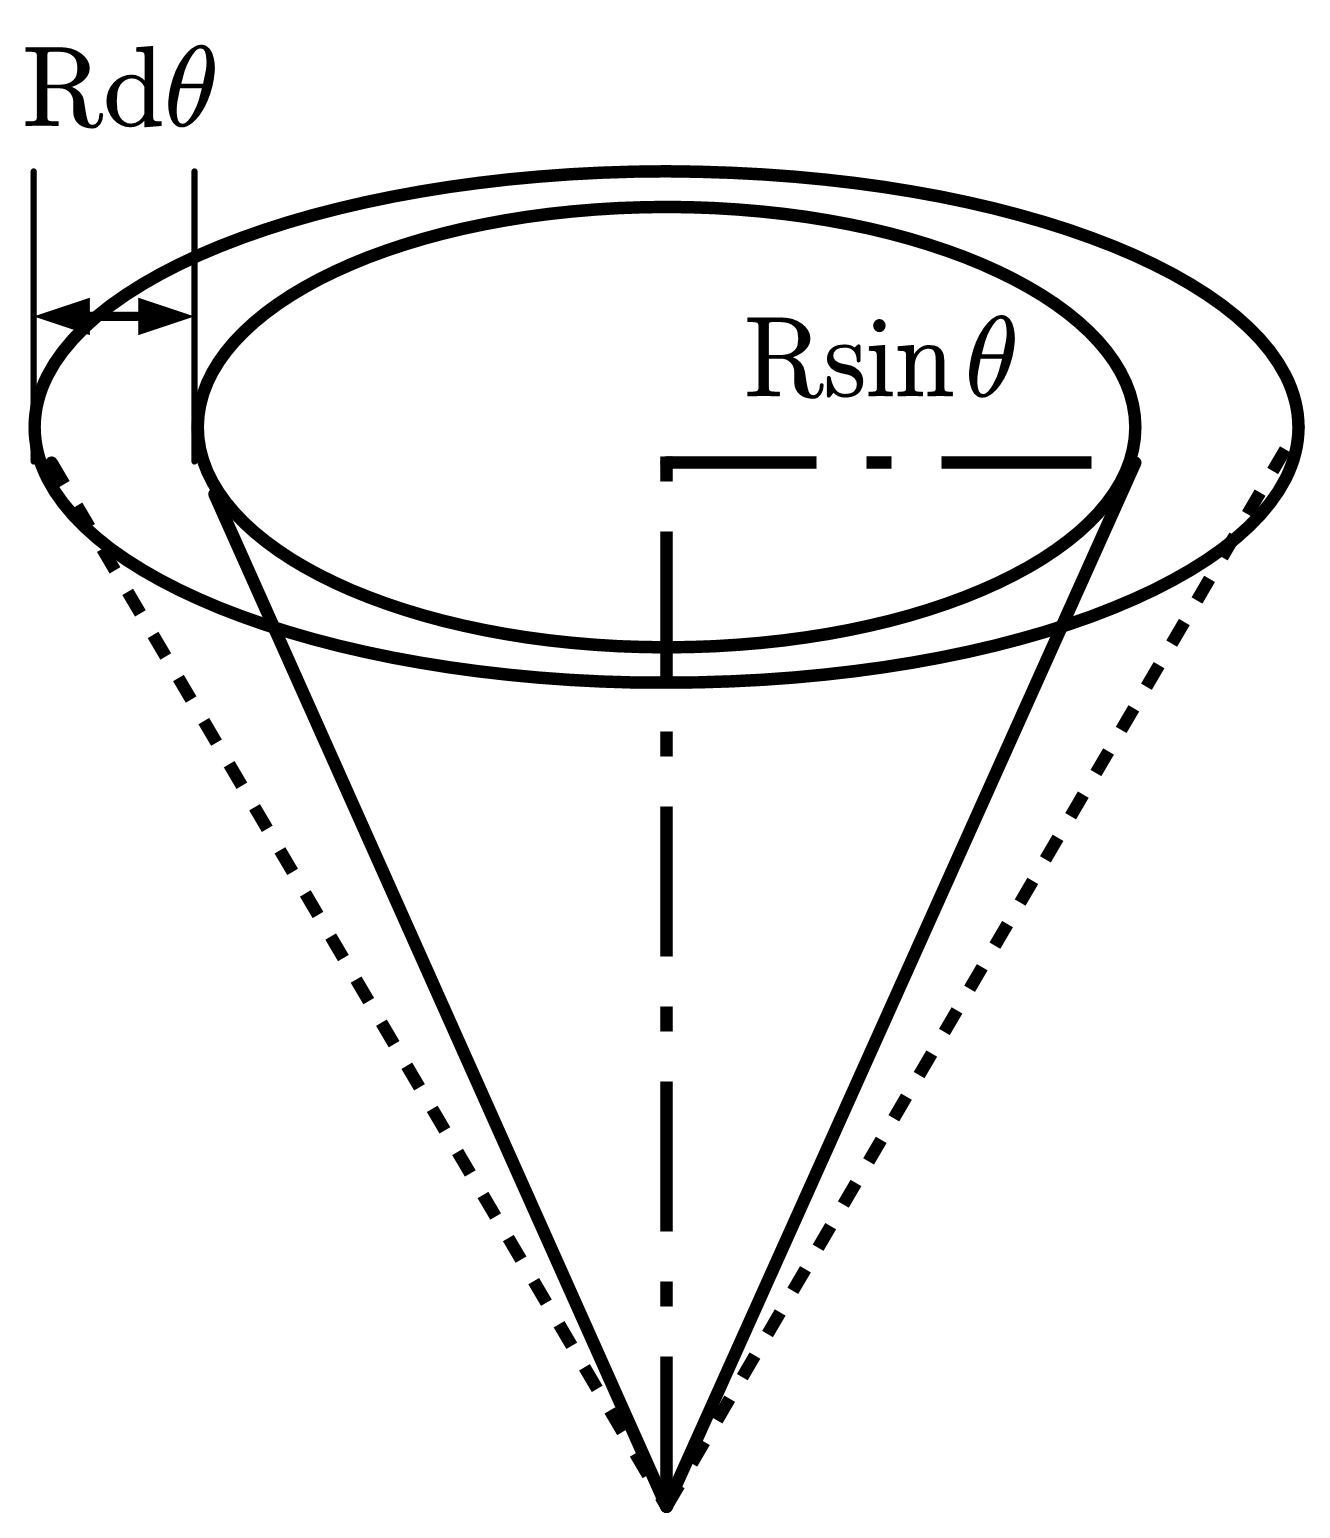
\includegraphics[width=4cm]{figure/NdThetaDist.png}
\end{center}
\subsubsection{常见情形下距离的分布}
\paragraph*{线段}在线段$[0,1]$上随机取2个点,计算距离的分布。

\begin{empheq}{align*}
\Prob(D\leq d)&=\Prob(|x-y|\leq d)\\
&=\Prob(x-d\leq y\leq x+d)
\end{empheq}

对应到正方形中对角梯形的面积,为
$$2\times \frac{\sqrt{2}+\sqrt{2}(1-d)}{2}\frac{d}{\sqrt{2}}=d(2-d)$$

\paragraph*{正方形}在矩形$[0,1]\times[0,1]$上随机取2个点,计算距离的分布。这个就非常复杂了。

